\documentclass[11pt]{article}

\usepackage[a4paper,margin=1in]{geometry}
\usepackage{graphicx}
\usepackage{hyperref}
\usepackage[T1]{fontenc}
\usepackage{lmodern}
\usepackage{microtype}

\graphicspath{{assets/generated/}}
\newcommand{\ExerciseTwoTrainSize}{3072}
\newcommand{\ExerciseTwoValSize}{1536}
\newcommand{\ExerciseTwoTestSize}{320}
\newcommand{\ExerciseTwoEpochs}{500}
\newcommand{\ExerciseTwoArchitecture}{a fully connected MLP with 6 hidden layers of width 12, input $(x_1,x_2,t)$, two outputs, and \texttt{tanh} activations}
\newcommand{\DiffusionWassersteinTwoD}{0.2876}
\newcommand{\FlowWassersteinTwoD}{0.2335}
\newcommand{\BetterMethodTextTwoD}{In this baseline, flow matching achieved the lower test-set Wasserstein distance.}


\begin{document}

\begin{center}
  {\large Data-Driven Methods in Engineering\par}
  \vspace{0.5em}
  {\LARGE\bfseries Diffusion Models and Flow Matching\par}
  \vspace{0.35em}
  {\large Minimal baseline answers for Exercise 2\par}
  \vspace{0.35em}
  {NTUA School of Civil Engineering\par}
\end{center}
\vspace{0.6em}

This document reports a minimal worked baseline for Exercise 2 only. Exercise 1 is intentionally left unanswered here.

The synthetic 2D swirl dataset used \ExerciseTwoTrainSize\ training samples, \ExerciseTwoValSize\ validation samples, and \ExerciseTwoTestSize\ test samples. Both methods use \ExerciseTwoArchitecture\ and were trained for \ExerciseTwoEpochs\ epochs.

\begin{figure}[t]
  \centering
  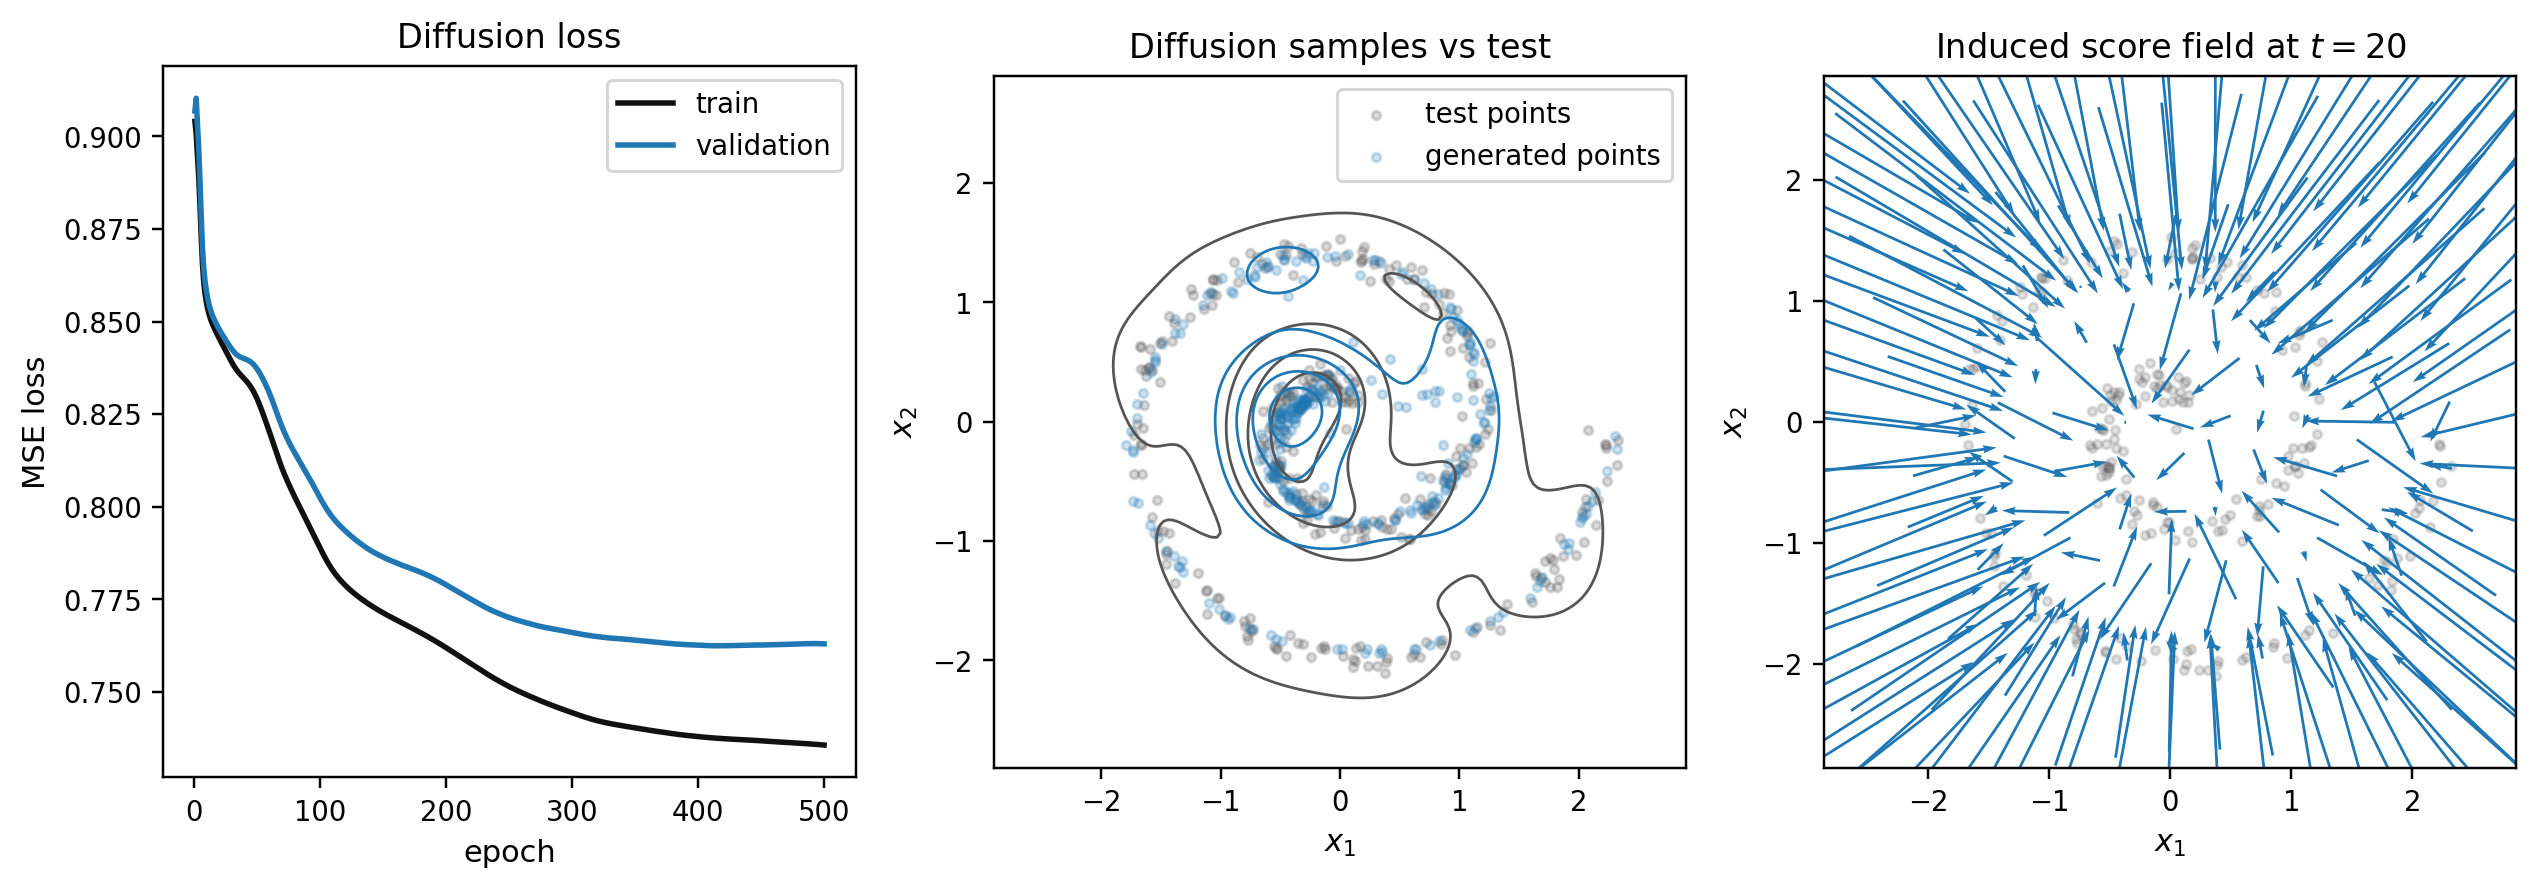
\includegraphics[width=\textwidth]{exercise2_diffusion_answer.png}
  \caption{Diffusion baseline: loss curves, generated-vs-test 2D sample comparison, and induced score estimate $\hat{s}_\theta(x_t,t)=-\varepsilon_\theta(x_t,t)/\sigma_t$.}
\end{figure}

\noindent\textbf{Diffusion test Wasserstein distance:} \DiffusionWassersteinTwoD.

\begin{figure}[t]
  \centering
  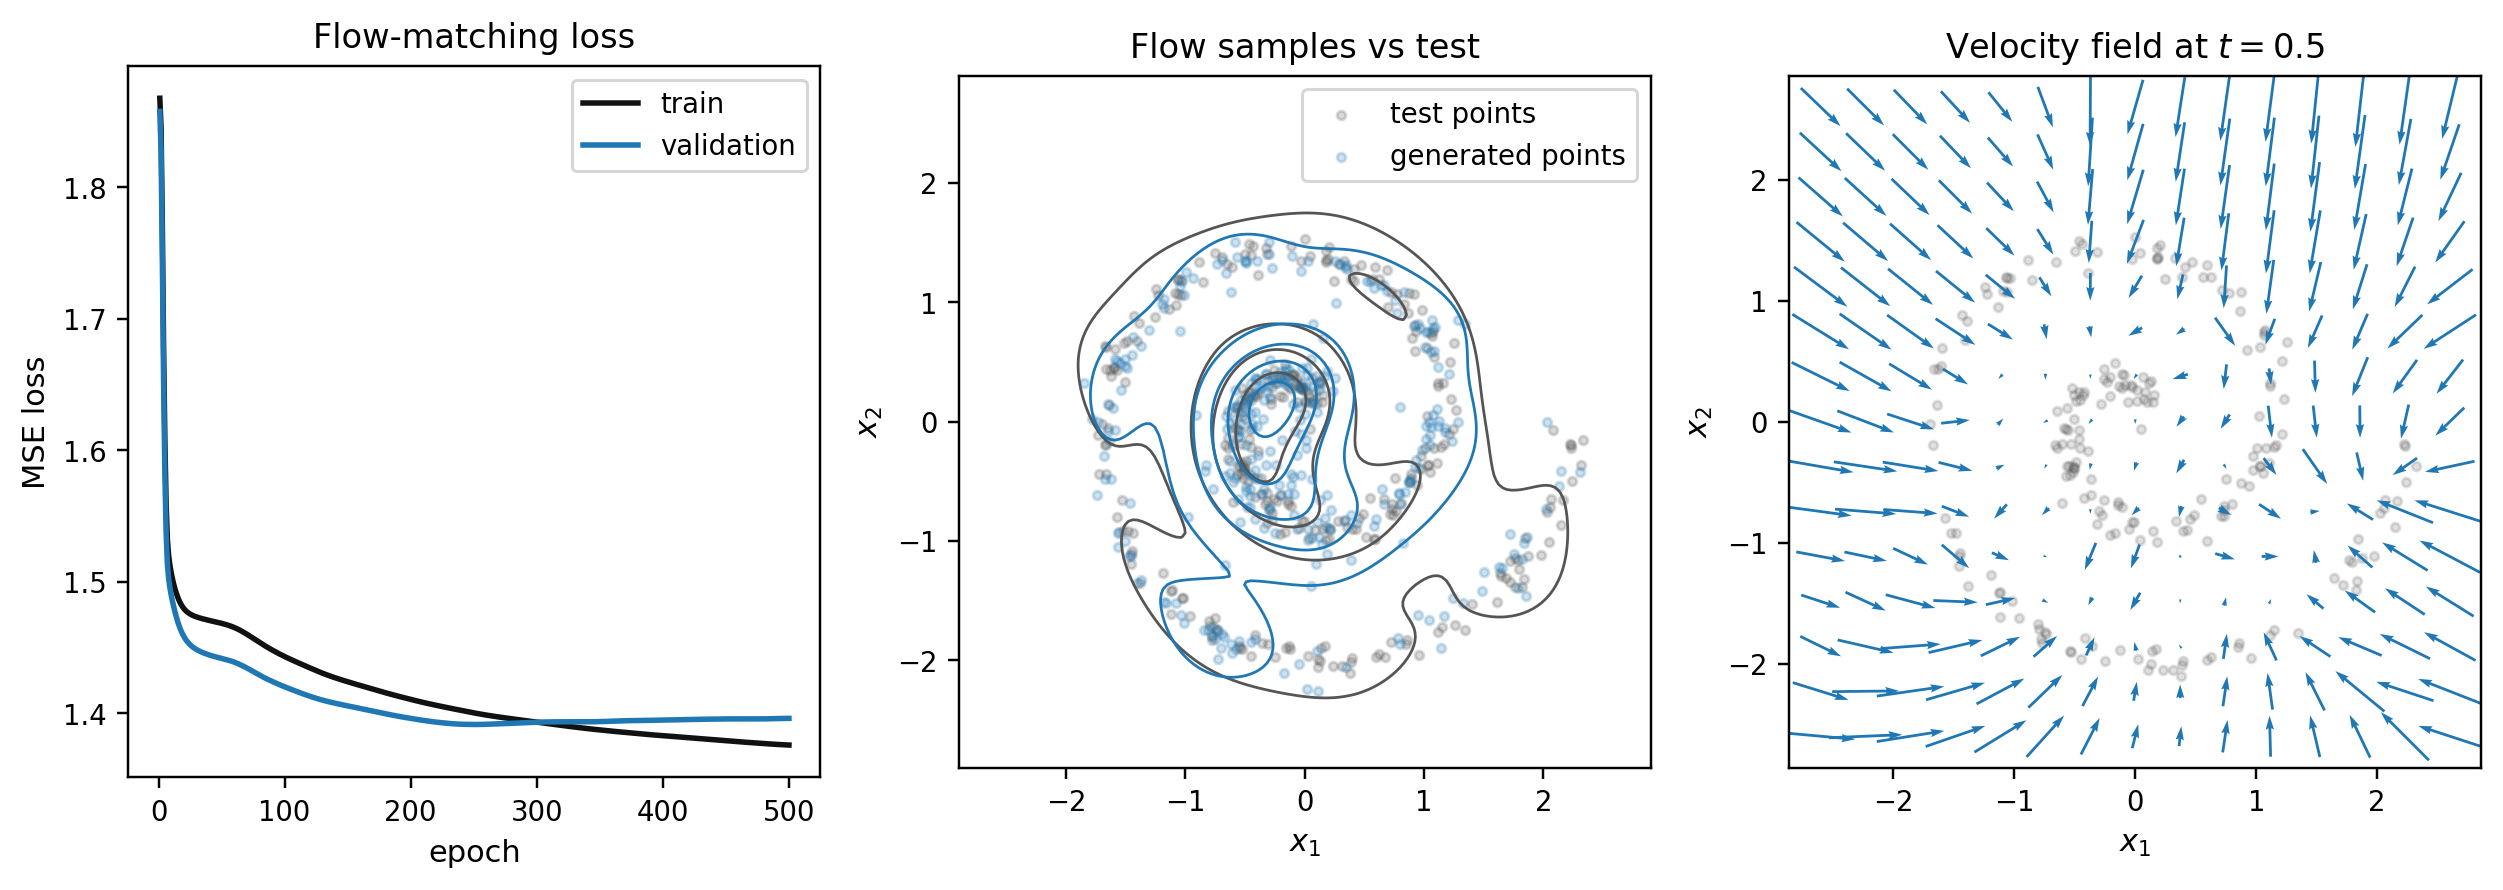
\includegraphics[width=\textwidth]{exercise2_flow_answer.png}
  \caption{Flow-matching baseline: loss curves, generated-vs-test 2D sample comparison, and the learned velocity vector field at a representative time; sampling uses Runge--Kutta integration.}
\end{figure}

\noindent\textbf{Flow-matching test Wasserstein distance:} \FlowWassersteinTwoD.

\paragraph{Comparison.}
\BetterMethodTextTwoD

\end{document}
